% Generated by python manage.py maps; text stays in LaTeX.
\begin{figure*}[p]
\centering
\begingroup
\setlength{\tabcolsep}{2pt}
\renewcommand{\arraystretch}{1}
\begin{tabular}{@{}cccc@{}}
\begin{minipage}[t]{0.205\textwidth}\vspace{0pt}\centering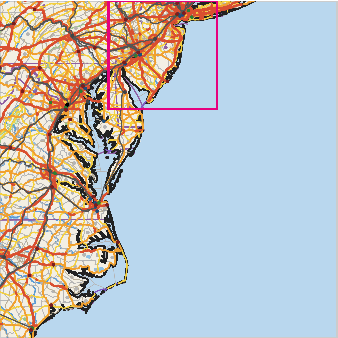
\includegraphics[width=\linewidth]{figures/map_natural_earth_vector_z5.pdf}\par\vspace{1pt}\scriptsize $z=5$\end{minipage} & \begin{minipage}[t]{0.205\textwidth}\vspace{0pt}\centering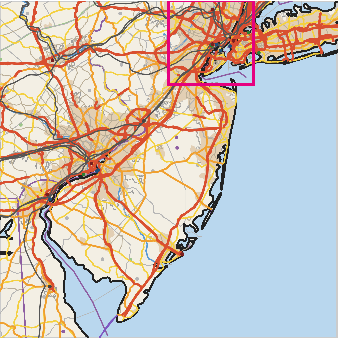
\includegraphics[width=\linewidth]{figures/map_natural_earth_vector_z7.pdf}\par\vspace{1pt}\scriptsize $z=7$\end{minipage} & \begin{minipage}[t]{0.205\textwidth}\vspace{0pt}\centering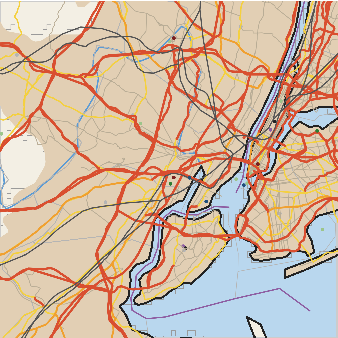
\includegraphics[width=\linewidth]{figures/map_natural_earth_vector_z9.pdf}\par\vspace{1pt}\scriptsize $z=9$\end{minipage} & \begin{minipage}[t]{0.34\textwidth}\vspace{1pt}\footnotesize\raggedright \textbf{(a) Natural Earth}\\ New York / New Jersey.\par\smallskip Colors are illustrative: blue water, pale land, tan urban areas, green parks, red/orange/yellow roads, purple state boundaries and gray county boundaries. Points mark places and transport facilities. Source: Natural Earth / NACIS.\end{minipage} \\[5pt]
\begin{minipage}[t]{0.205\textwidth}\vspace{0pt}\centering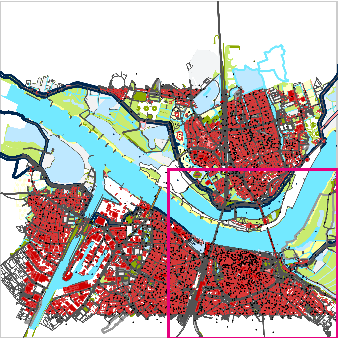
\includegraphics[width=\linewidth]{figures/map_pdok_netherlands_infrostructure_z12.pdf}\par\vspace{1pt}\scriptsize $z=12$\end{minipage} & \begin{minipage}[t]{0.205\textwidth}\vspace{0pt}\centering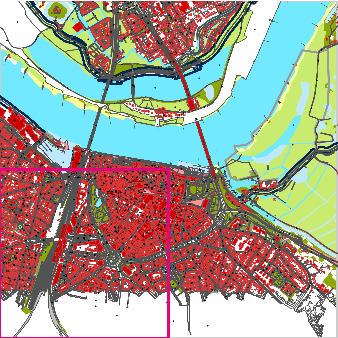
\includegraphics[width=\linewidth]{figures/map_pdok_netherlands_infrostructure_z13.pdf}\par\vspace{1pt}\scriptsize $z=13$\end{minipage} & \begin{minipage}[t]{0.205\textwidth}\vspace{0pt}\centering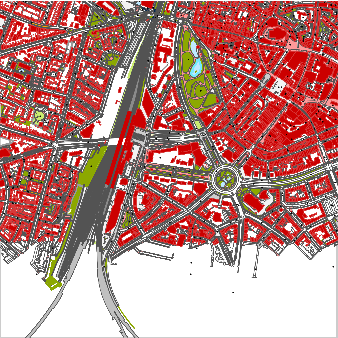
\includegraphics[width=\linewidth]{figures/map_pdok_netherlands_infrostructure_z14.pdf}\par\vspace{1pt}\scriptsize $z=14$\end{minipage} & \begin{minipage}[t]{0.34\textwidth}\vspace{1pt}\footnotesize\raggedright \textbf{(b) PDOK BGT}\\ Nijmegen, Netherlands.\par\smallskip The palette follows the BGT standard visualization: red buildings, blue water, green vegetation and white local roads/paved areas; gray denotes classes without an assigned standard color. Source: PDOK.\end{minipage} \\[5pt]
\begin{minipage}[t]{0.205\textwidth}\vspace{0pt}\centering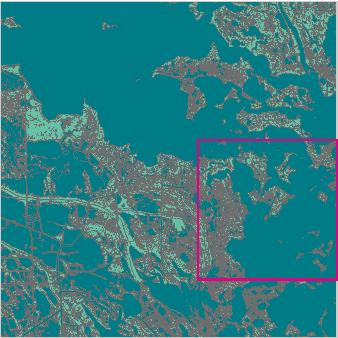
\includegraphics[width=\linewidth]{figures/map_usfws_luisiana_wetlands_geopackage_z10.pdf}\par\vspace{1pt}\scriptsize $z=10$\end{minipage} & \begin{minipage}[t]{0.205\textwidth}\vspace{0pt}\centering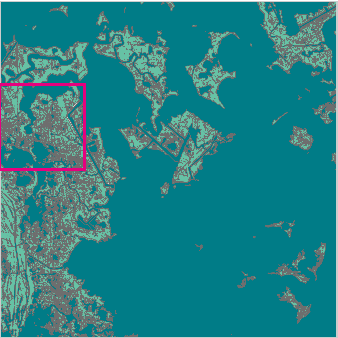
\includegraphics[width=\linewidth]{figures/map_usfws_luisiana_wetlands_geopackage_z12.pdf}\par\vspace{1pt}\scriptsize $z=12$\end{minipage} & \begin{minipage}[t]{0.205\textwidth}\vspace{0pt}\centering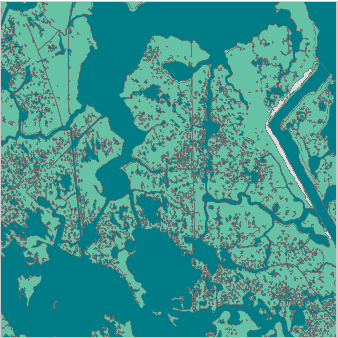
\includegraphics[width=\linewidth]{figures/map_usfws_luisiana_wetlands_geopackage_z14.pdf}\par\vspace{1pt}\scriptsize $z=14$\end{minipage} & \begin{minipage}[t]{0.34\textwidth}\vspace{1pt}\footnotesize\raggedright \textbf{(c) USFWS wetlands}\\ coastal Louisiana.\par\smallskip The NWI palette distinguishes forested/shrub wetlands (dark green), emergent wetlands (light green), tidal wetlands (teal), and water classes (blue); unclassified polygons are light gray. Source: U.S. Fish and Wildlife Service, National Wetlands Inventory.\end{minipage} \\[5pt]
\begin{minipage}[t]{0.205\textwidth}\vspace{0pt}\centering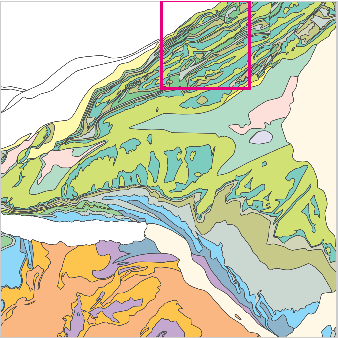
\includegraphics[width=\linewidth]{figures/map_swisstopo_mountains_vector_z10.pdf}\par\vspace{1pt}\scriptsize $z=10$\end{minipage} & \begin{minipage}[t]{0.205\textwidth}\vspace{0pt}\centering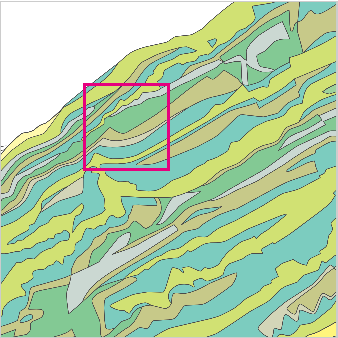
\includegraphics[width=\linewidth]{figures/map_swisstopo_mountains_vector_z12.pdf}\par\vspace{1pt}\scriptsize $z=12$\end{minipage} & \begin{minipage}[t]{0.205\textwidth}\vspace{0pt}\centering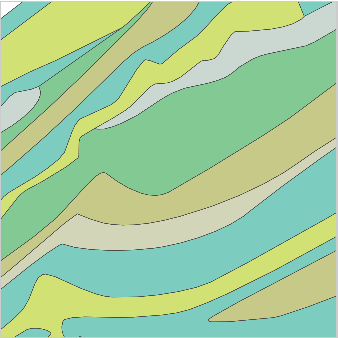
\includegraphics[width=\linewidth]{figures/map_swisstopo_mountains_vector_z14.pdf}\par\vspace{1pt}\scriptsize $z=14$\end{minipage} & \begin{minipage}[t]{0.34\textwidth}\vspace{1pt}\footnotesize\raggedright \textbf{(d) swisstopo geology}\\ Saentis, Switzerland.\par\smallskip Colors distinguish geological units using the swisstopo legend and the retained \texttt{SYMBOL}/\texttt{INDEX\_} attributes. White denotes units without an assigned legend color. Source: swisstopo, Structural Map of the Helvetic Zone, sheet 128.\end{minipage} \\[5pt]
\begin{minipage}[t]{0.205\textwidth}\vspace{0pt}\centering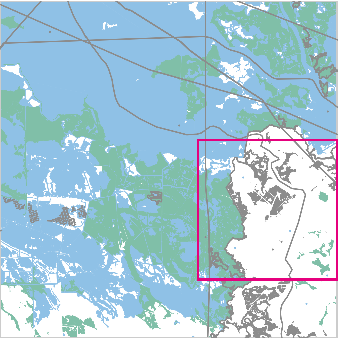
\includegraphics[width=\linewidth]{figures/map_louisiana-260912_z10.pdf}\par\vspace{1pt}\scriptsize $z=10$\end{minipage} & \begin{minipage}[t]{0.205\textwidth}\vspace{0pt}\centering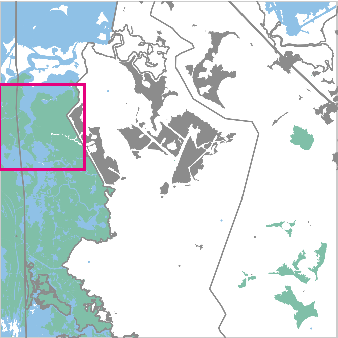
\includegraphics[width=\linewidth]{figures/map_louisiana-260912_z12.pdf}\par\vspace{1pt}\scriptsize $z=12$\end{minipage} & \begin{minipage}[t]{0.205\textwidth}\vspace{0pt}\centering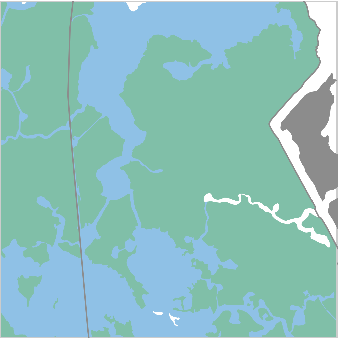
\includegraphics[width=\linewidth]{figures/map_louisiana-260912_z14.pdf}\par\vspace{1pt}\scriptsize $z=14$\end{minipage} & \begin{minipage}[t]{0.34\textwidth}\vspace{1pt}\footnotesize\raggedright \textbf{(e) OpenStreetMap}\\ coastal Louisiana.\par\smallskip An illustrative tag-based palette shows water in blue, wetlands in teal, vegetation in green, buildings in brown, roads/routes in orange and other objects in gray. Classification uses retained OSM tags rather than merged tile-layer names. Source: \copyright{} OpenStreetMap contributors, ODbL.\end{minipage} \\[5pt]
\end{tabular}
\endgroup
\caption{The five datasets at three zoom levels, rendered from Standard MVT tiles. Views are nested from left to right; magenta outlines locate the next view. Square viewports stay within the configured data bounds at each zoom. USFWS and OSM show the same coastal Louisiana areas.}
\label{fig:datasets}
\label{fig:map-natural_earth_vector}
\label{fig:map-pdok_netherlands_infrostructure}
\label{fig:map-usfws_luisiana_wetlands_geopackage}
\label{fig:map-swisstopo_mountains_vector}
\label{fig:map-louisiana-260912}
\end{figure*}
